\documentclass[specification,annotation,times]{itmo-student-thesis}
%% \documentclass[times]{itmo-student-thesis}

%% Опции пакета:
%% - specification - если есть, генерируется задание, иначе не генерируется
%% - annotation - если есть, генерируется аннотация, иначе не генерируется
%% - times - делает все шрифтом Times New Roman, собирается с помощью xelatex
%% - pscyr - делает все шрифтом Times New Roman, требует пакета pscyr.

%% Делает запятую в формулах более интеллектуальной, например:
%% $1,5x$ будет читаться как полтора икса, а не один запятая пять иксов.
%% Однако если написать $1, 5x$, то все будет как прежде.
\usepackage{icomma}

%% Один из пакетов, позволяющий делать таблицы на всю ширину текста.
\usepackage{tabularx}

%% Мульти-иллюстрации
\usepackage[caption=false,font=footnotesize]{subfig}

%% Данные пакеты необязательны к использованию в бакалаврских/магистерских
%% Они нужны для иллюстративных целей
%% Начало
\usepackage{tikz}
\usetikzlibrary{arrows}
%% Конец

%% Указываем файл с библиографией.
\addbibresource{master-thesis.bib}

%% Указываем путь к иллюстрациям
\graphicspath{{img/}{live_img/}}

%% Шорткаты
\DeclareMathOperator{\argmin}{argmin}
\DeclareMathOperator{\argmax}{argmax}

%% Теоремы/определения
\theoremstyle{definition}

\newtheorem{definition-ru}{Определение}

\begin{document}

\studygroup{M4239}
\title{Децентрализованный алгоритм управления конвейерной системой с использованием методов мультиагентного обучения с подкреплением}
\author{Мухутдинов Дмитрий Вадимович}{Мухутдинов Д.В.}
\supervisor{Фильченков Андрей Александрович}{Фильченков А.А.}{к.ф-м.н.}{кафедра КТ}
\publishyear{2019}
%% Дата выдачи задания. Можно не указывать, тогда надо будет заполнить от руки.
\startdate{01}{сентября}{2017}
%% Срок сдачи студентом работы. Можно не указывать, тогда надо будет заполнить от руки.
\finishdate{31}{мая}{2019}
%% Дата защиты. Можно не указывать, тогда надо будет заполнить от руки.
\defencedate{07}{июня}{2019}

\addconsultant{Вяткин В.В.}{проф., д.т.н.}

\secretary{Павлова О.Н.}

%% Задание
%%% Техническое задание и исходные данные к работе
\technicalspec{Требуется разработать децентрализованный алгоритм управления
  конвейерной системы для транспортировки багажа. Алгоритм должен позволять
  контроллерам конвейерной сети динамически изменять свое поведение в целях
  адаптации под изменившиеся условия работы, такие как поломка одного из
  конвейеров или изменение интенсивности потока багажа. Алгоритм должен
  обеспечивать своевременную доставку багажных единиц до пунктов назначения, в
  то же время минимизируя энергопотребление всей системы в целом.
}

%%% Содержание выпускной квалификационной работы (перечень подлежащих разработке вопросов)
\plannedcontents{Пояснительная записка должна содержать обзор существующих
  результатов в сфере управления конвейерными системами, а также в сферах,
  имеющих непосредственное отношение к предложенному алгоритму (таких как
  сетевая маршрутизация и обучение с подкреплением). Также записка должна
  содержать подробное изложение предложенного алгоритма и данные
  экспериментального сравнения его производительности с производительностью
  существующих методов управления конвейерной системой, проведенного с помощью
  виртуальной имитационной модели конвейерной сети.
}

%%% Исходные материалы и пособия 
\plannedsources{\begin{enumerate}
  \item Richard S. Sutton and Andrew G. Barto. Reinforcement Learning: An Introduction. The MIT Press, 2012
  \item Mnih et al. Human-level control through deep reinforcement learning. Nature, 518(7540):529–533, 2015.
\end{enumerate}}

%%% Цель исследования
\researchaim{
  Разработка децентрализованного алгоритма управления конвейерной системой,
  способного адаптироваться к гетерогенным изменениям в условиях работы.
}

%%% Задачи, решаемые в ВКР
\researchtargets{\begin{enumerate}
    \item разработка виртуальной имитационной модели конвейерной сети,
      позволяющей проводить сравнительный анализ алгоритмов управления;
    \item реализация ряда известных алгоритмов управления конвейерной сетью (а
      также маршрутизации) в рамках разработанной имитационной модели;
    \item разработка алгоритма, соответствующего поставленным требованиям;
    \item экспериментальное сравнение разработанного алгоритма с существующими
      по качеству работы.
\end{enumerate}}

%%% Использование современных пакетов компьютерных программ и технологий
\addadvancedsoftware{Язык программирования Python 3.6}{Гл. \ref{experiments};
  приложения \ref{apx:bad-results}, \ref{apx:simulators}}
\addadvancedsoftware{Библиотека для дискретно-событийного моделирования SimPy}{Гл. \ref{experiments};
  приложения \ref{apx:bad-results}, \ref{apx:simulators}}
\addadvancedsoftware{Библиотека для операций с графами NetworkX}{Гл. \ref{experiments};
  приложения \ref{apx:bad-results}, \ref{apx:simulators}}
\addadvancedsoftware{Математические пакеты NumPy и SciPy}{Гл. \ref{experiments};
  приложения \ref{apx:bad-results}, \ref{apx:simulators}}
\addadvancedsoftware{Библиотеки для машинного обучения scikit-learn и PyTorch}{Гл. \ref{experiments};
  приложения \ref{apx:bad-results}, \ref{apx:simulators}}
\addadvancedsoftware{Среда интерактивной разработки Jupyter Lab}{Гл. \ref{experiments};
  приложения \ref{apx:bad-results}, \ref{apx:simulators}}
\addadvancedsoftware{Библиотеки Matplotlib, Seaborn и Pandas для обработки и визуализации данных}{Гл. \ref{experiments};
  приложения \ref{apx:bad-results}, \ref{apx:simulators}}

%%% Краткая характеристика полученных результатов 
\researchsummary{
  Разработан алгоритм управления конвейерной системой на основе глубокого
  мультиагентного обучения с подкреплением. В ходе экспериментального
  исследования было установлено, что разработанный алгоритм превосходит
  существующие по качеству работы и способен адаптироваться к изменениям во
  внешней среде.
}

%%% Гранты, полученные при выполнении работы 
\researchfunding{
  Государственное задание № 2.8866.2017/БЧ <<Технология разработки программного
  обеспечения систем управления ответственными объектами на основе глубокого
  обучения и конечных автоматов>>
}

%%% Наличие публикаций и выступлений на конференциях по теме выпускной работы
\researchpublications{
\begin{refsection}
\nocite{mukhutdinov2019multi}
\nocite{mukhutdinov2019kmu}
\printannobibliography
\end{refsection}
}

%% Эта команда генерирует титульный лист и аннотацию.
\maketitle{Магистр}

%% Оглавление
\tableofcontents

%% Макрос для введения. Совместим со старым стилевиком.
\startprefacepage

Конвейерные системы широко применяются для автоматизированной транспортировки
объектов и материалов. Они являются неотъемлемой частью комплексов промышленного
оборудования, пунктов сортировки грузов, багажных систем в аэропортах и т. д..
Оптимизация работы таких системы имеет высокую практическую и экономическую
значимость, что мотивирует поиск эффективных методов управления конвейерными
системами.

Для управления большинством современных конвейерных систем применяются
централизованные статические стратегии управления, специально разрабатываемые
под конкретную систему одновременно с проектированием ее физической топологии в
целях решения задач конкретного предприятия \cite{de1994baggage}. Преимуществами
такого подхода являются высокая производительность работы и предсказуемость
поведения системы. Недостатками такого подхода являются высокая стоимость и
долгие сроки разработки кастомизированной стратегии управления, неспособность
системы адаптироваться к изменениям во внешний условиях, не учтенных во время
проектирования (таким как неожиданный отказ отдельных элементов системы), а
также наличие централизованного контроллера как критической точки отказа.

В связи с обозначенными недостатками использования кастомизированных стратегий
управления существует интерес к разработке обобщенных систематических подходов к
управлению конвейерными системами. Наиболее популярным подходом из используемых
является управление с прогнозируемыми моделями (\textit{англ.} model predictive
control, MPC) \cite{qin2003survey}. Управление с прогнозируемыми моделями
изначально разрабатывалось для задач химической промышленности и
нефтепереработки \cite{eaton1992model}, и на данный момент широко используется в
этих сферах. В последние несколько лет повысился интерес к применению данного
подхода к управлению другими типами киберфизических систем, в том числе
промышленными конвейерными линиями \cite{cataldo2016dynamic, luo2015energy} и
системами распределения багажа на основе рельсовых тележек (\textit{англ.}
destination coded vehicles, DCVs) \cite{tarau2010model, zeinaly2015integrated}.
Существующие алгоритмы на основе управления с прогнозируемыми моделями
обобщаются на различные конкретные конфигурации физических систем, но все еще
предусматривают наличие централизованного контроллера. Кроме того, модификация
существующего алгоритма управления (например, добавления учета энергопотребления
системы) во многих случаях является нетривиальной задачей, так как
оптимизируемая функция во фреймворке MPC должна выражаться как задача линейного
(\textit{англ.} linear programming, LP) или квадратичного программирования
(\textit{англ.} quadratic programming, QP). В связи с этим существует интерес к
разработке иных, децентрализованных подходов к управлению конвейерными сетями,
требующих менее строгих ограничений к характеру решаемой задачи.

При рассмотрении штучных конвейеров, перемещающих отдельные объекты, как в
случае систем для перемещения багажа в аэропортах, задача управления конвейерной
системой по большей части сводится к задаче пакетной маршрутизации
(\textit{англ.} packet routing). Задача пакетной маршрутизации --- это задача
поиска пути наименьшей стоимости в графе из текущей вершины $n$ в вершину
назначения $d$. В контексте конвейерных систем топология конвейерной сети может
быть представлена в виде ориентированного графа, а перемещаемые по конвейерам
объекты могут быть абстрагированы как <<пакеты>>. 

Задача пакетной маршрутизации впервые обрела актуальность с появлением
компьютерных сетей. Первые алгоритмы сетевой маршрутизации появились в процессе
разработки сети ARPANet. Именно тогда были изобретены такие подходы к пакетной
маршрутизации, как дистанционно-векторный (\textit{англ.} distance-vector)
\cite{arpanet-orig} и состояния каналов связи (\textit{англ.} link-state)
\cite{link-state-arpanet}, которые и по сей день лежат в основе
таких стандартных и широко применяемых алгоритмов сетевой маршрутизации, как
Routing Information Protocol (RIP) \cite{rip-rfc} и Open Shortest Path First
(OSPF) \cite{ospf-rfc}. Преимуществами алгоритмов сетевой маршрутизации являются
обусловленные характером задачи децентрализованность, низкая требовательность к
вычислительным ресурсам и устойчивость к отказам маршрутизаторов и обрывам
соединений. В работе \cite{vyatkin-controllers} было продемонстрировано, что
простой дистанционно-векторный алгоритм маршрутизации может быть напрямую
применен к задаче управления конвейерной системой для транспортировки багажа,
что позволяет достигнуть устойчивости системы к отказам отдельных конвейеров.
Однако, в силу своей простоты, дистанционно-векторный алгоритм решает
исключительно задачу направления перемещаемых объектов вдоль кратчайших путей в
конвейерной сети, что ограничивает его применимость в тех случаях, когда
необходимо учитывать дополнительные критерии оптимизации (такие как
энергопотребление системы).

Cуществуют и другие подходы к решению задачи пакетной маршрутизации. Одним из
таких подходов является подход на основе идеи обучения с подкреплением
(\textit{англ.} reinforcement learing, RL). Первым таким алгоритмом стал алгоритм
Q-routing \cite{q-routing-orig}, основанный на методе Q-learning
\cite{q-learning-orig}. Этот алгоритм, как и его модификации
\cite{predictive-q-routing, dual-q-routing}, благодаря обучению с подкреплением
оказался способен лучше адаптироваться к изменениям в интенсивности сетевого
трафика, чем алгоритмы, основанные на вычислении кратчайшего пути. Но из-за
использования большого количества служебных сообщений, использующих те же каналы
передачи данных, что и целевые пакеты, применение таких алгоритмов в реальных
компьютерных сетях ограничено.

В контексте конвейерных сетей, однако, целевые <<пакеты>> являются физическими
объектами (например, чемоданами), перемещаемыми по конвейерной ленте, в то время
как служебные сообщения передаются по проводным соединениям между контроллерами.
Таким образом, время распространения служебных сообщений по системе пренебрежимо
мало по сравнению с временем перемещения целевых объектов, что нивелирует
озвученный недостаток алгоритмов маршрутизации, основанных на обучении с
подкреплением.

В данной работе будет предложено несколько модификаций децентрализованного
алгоритма управления конвейерной системой, основанного на методе Q-routing, но
использующего нейронную сеть в качестве обучающегося агента. Для демонстрации
способности работы алгоритма в различных постановках задачи маршрутизации он
будет исследован как в имитационной модели конвейерной системы, так и в
имитационной модели абстрактной компьютерной сети.

В главе 1 будут рассмотрены существующие подходы к управлению конвейерными
системами и маршрутизации. Также будет сформулирована обобщенная постановка
задачи маршрутизации в терминах мультиагентного обучения с подкреплением, к
которой будет сведена задача управления конвейерной системой. Будут рассмотрены
существующие алгоритмы маршрутизации, их сильные и слабые стороны. Также будут
рассмотрены существующие методы обучения нейронных сетей с подкреплением, в том
числе в мультиагентном случае.

В главе 2 будет рассмотрен предложенный алгоритм и его модификации и обоснованы
решения, принятые в ходе его разработки.

В главе 3 будут приведены экспериментальные результаты работы алгоритма для
задач пакетной маршрутизации в моделях компьютерной сети и управления системой багажных
конвейеров. Также будет проведено экспериментальное сравнение алгоритма с
существующими алгоритмами маршрутизации и управления конвейерной системой.

%% Начало содержательной части.
\chapter{Обзор предметной области}

%% Так помечается начало обзора.
\startrelatedwork

\section{Методы управления киберфизическими системами}

\begin{definition-ru}
  \textbf Управление с прогнозируемыми моделями (\textit{англ.} model predictive
  control, MPC) --- это...
\end{definition-ru}

TBD

\section{Алгоритмы пакетной маршрутизации}

Почти все существующие алгоритмы пакетной маршрутизации были разработаны для
маршрутизации пакетов в компьютерных сетях. Большинство алгоритмов маршрутизации
в компьютерных сетях, применяемых на практике, относятся к одному из двух
семейств алгоритмов --- дистанционно-векторные (distance-vector) \cite{arpanet-orig} или
состояния каналов связи (link-state) \cite{link-state-arpanet}.
Концептуально все алгоритмы внутри каждого из этих семейств одинаковы, и различаются только
техническими деталями реализации, обусловленными спецификой конкретной узкой
сферы применения. Поэтому мы не будем рассматривать алгоритмы каждого семейства
по отдельности, а рассмотрим только концепции в целом.

\subsection{Дистанционно-векторные алгоритмы}

Идея дистанционно-векторных алгоритмов (distance-vector algoritms) заключается в
следующем:

\begin{itemize}
\item Каждый маршрутизатор $s$ в сети хранит таблицу, в которой для каждого другого узла
  сети $d$ хранится следующая информация:
  \begin{itemize}
  \item Предполагаемое кратчайшее расстояние от $s$ до $d$
  \item Сосед $n$, которому нужно отправить пакет, чтобы пакет прошел по
    кратчайшему пути до узла $d$.
  \end{itemize}
\item Периодически каждый маршрутизатор рассылает свою версию таблицы кратчайших
  расстояний всем своим соседям
\item При получении вектора кратчайших расстояний от соседа маршрутизатор $s$
  сравнивает его поэлементно с текущей версией. Если оказывается, что наименьшая
  стоимость пути от соседа $n$ до узла $d$, сложенная c оценкой стоимости ребра
  $(s, d)$ меньше, чем наименьшая стоимость пути от $s$ до $d$ в текущей
  таблице, то значение в текущей таблице обновляется, и наилучшим соседом для
  отправки пакета в узел $d$ становится сосед $n$.
\end{itemize}

Как можно видеть, дистанционно-векторный алгоритм является, в сущности,
распределенной версией алгоритма Беллмана-Форда поиска кратчайшего пути в
графе \cite{bellman-ford}.

Различные реализации дистанционно-векторного метода различаются, в частности,
оценками стоимости соединений в сети. Так, например, протокол RIP \cite{rip-rfc} просто
оценивает стоимость каждого соединения в 1, а IGRP \cite{igrp-patent} оценивает
стоимость соединений исходя из оценок задержки и пропускной способности.

Преимуществами дистанционно-векторных алгоритмов являются простота реализации и
низкие требования к памяти и вычислительной мощности. Недостатками же являются
низкая скорость распространения информации по сети и сложности с приспособлением
под изменяющуюся топологию (проблема count-to-infinity). Этих проблем
удается избежать при применении другого распространенного подхода --- алгоритмов
на основе состояния канала связи. 

\subsection{Алгоритмы состояния канала связи}

В отличие от дистанционно-векторных алгоритмов, в алгоритмах состояния канала связи
(link-state) каждый узел сети хранит у себя модель всей сети в виде графа.
Рассмотрим шаги алгоритма подробнее:

\begin{itemize}
\item Каждый маршрутизатор периодически проверяет состояние соединений до
  соседей
\item При обнаружении обрыва какого-либо соединения алгоритм удаляет это
  соединение из собственного графа и рассылает соседям новую версию состояния
  соединений до них
\item Соседи обновляют собственные версии графов в соответствии с полученной
  информацией и пересылают сообщение дальше
\item Чтобы избежать зацикливания сообщений об обновлении состояния, каждое
  сообщение снабжается \textit{номером версии}. Маршрутизатор $n$ игнорирует
  сообщение от маршрутизатора $n$, если номер версии этого сообщения меньше или
  равен предыдущему.
\end{itemize}

Имея информацию обо всей сети в целом, маршрутизатор может рассчитать кратчайшие
пути до всех остальных узлов. Обычно для этого используется алгоритм
Дейкстры \cite{dijkstra}. 

Link-state алгоритмы обладают способностью адаптироваться под изменения
топологии сети гораздо быстрее, чем distance-vector алгоритмы за счет
несколько более сложной реализации и чуть больших затрат по памяти и
вычислительной мощности. Это обуславливает то, что на данный момент именно
link-state протоколы, такие как OSPF \cite{ospf-rfc}, доминируют в сетевой
маршрутизации. Однако даже в решении задачи сетевой маршрутизации link-state
алгоритмы в чистом виде не лучшим образом адаптируются к повышению нагрузки в
сети. Рассматриваемые в дальнейшем другие алгоритмы, основанные на принципе
обучения с подкреплением, справляются с задачей адаптации к
изменчивой нагрузке лучше.

\subsection{Q-routing}\label{q-routing-desc}

Среди других подходов особый интерес представляют подходы на основе обучения с
подкреплением. Первым алгоритмом маршрутизации, основанным на этой идее, стал
алгоритм Q-routing \cite{q-routing-orig}. Принцип его работы таков:

\begin{itemize}
\item Каждый маршрутизатор $x$ хранит $Q_x(d, y)$ --- оценку минимального
  времени в пути до узла $d$, если следующим узлом на пути является сосед $y$.
  Очевидно, что $\forall y : Q_x(x, y) = 0$ 
\item Пакет, который необходимо доставить в узел $d$, отправляется соседу
  $y = \argmin\limits_{(x, y) \in E} Q_x(d, y)$
\item При получении пакета узел $y$ отправляет узлу $x$ время получения $t_r$ и
  собственную оценку оставшегося времени в пути
  $t = \min\limits_{(y, z) \in E} Q_y(d, z)$
\item Зная время отправления пакета $t_s$ и получив $t_r$ и $t$, узел $x$
  обновляет собственную оценку по формуле:
  $Q_x(d, y) = \alpha((t_r - t_s) + t - Q_x(d, y)) + Q_x(d, y)$,
  где $\alpha$ --- это learning rate, параметр алгоритма.
\end{itemize}

Было показано, что этот алгоритм способен хорошо адаптироваться к изменениям в
топологии сети и интенсивности трафика. Такие его модификации, как dual
Q-routing \cite{dual-q-routing} и predictive Q-routing \cite{predictive-q-routing}
демонстрируют еще более высокое качество маршрутизации. Однако по сравнению с
distance-vector или link-state методами данные алгоритмы используют гораздо
больше служебных сообщений (служебный пакет на каждую пересылку целевого
пакета), что ограничивает их применение в реальных высоконагруженных
компьютерных сетях.

Однако в задачах маршрутизации вне контекста компьютерных сетей это перестает
быть проблемой, так как целевые \enquote{пакеты} (чемоданы на конвейере, автомобили на
автостраде, etc.) и служебные сообщения в таких задачах являются объектами разной природы и
передаются по разным каналам, причем служебные сообщения по сравнению с целевыми
\enquote{пакетами} доставляются мгновенно. Эти обстоятельства делают применение
алгоритмов обучения с подкреплением в таких задачах более привлекательным.

\subsection{Применение машинного обучения в сетевой маршрутизации}

TBD

\subsubsection{Программно-определяемые сети (SDN)}

TBD

\subsection{Другие подходы}

Для полноты обзора приведем еще несколько примеров.

Идея использования нейросетей для решения задачи маршрутизации не нова. В
работах \cite{ali-nn-routing, araujo2001neural} для решения задачи поиска кратчайшего пути в графе
используются нейронные сети Хопфилда. Однако, эти исследования преследовали цель
ускорения вычисления кратчайшего пути за счет аппаратной реализации нейросети,
что кардинально отличается от цели текущей работы.

Еще одним интересным подходом является AntNet \cite{di1998antnet}. Это алгоритм,
построенный на идее исследования состояния сети с помощью специальных
пакетов-\enquote{агентов}. Алгоритм показал хорошие результаты в ходе исследований, но
не получил широкого применения, вероятно, в силу уже массового к тому времени
распространения link-state и distance-vector протоколов.

\section{Применение обучения с подкреплением к поставленной задаче}

\subsection{Термины и понятия}

\begin{definition-ru}
  \textbf{Обучение с подкреплением} (\textit{англ.} reinforcement learning, RL) --- вид машинного
  обучения, в котором \textit{агент} (agent) каждый момент времени $t$ 
  взаимодействует со \textit{средой} (environment), находящейся в
  \textit{состоянии} (state) $s_t \in \mathcal{S}$ путем выбора
  \textit{действия} (action) $a \in \mathcal{A}_{s_t}$ и получения
  \textit{вознаграждения} (reward) $r_{t+1} \in \Bbb{R}$ c переходом в новое
  \textit{состояние} $s_{t+1}$.
\end{definition-ru}

\begin{figure}[!h]
  \caption{Схема взаимодействия агента и среды в обучении с подкреплением}\label{rl-scheme}
  \centering
  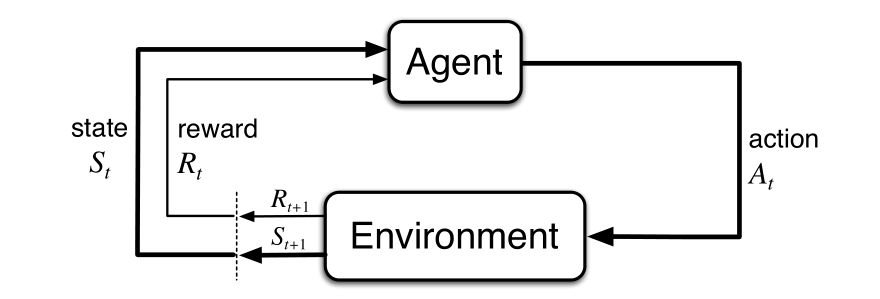
\includegraphics[scale=0.5]{rl-scheme}
\end{figure}

\begin{definition-ru}
  \textbf{Марковский процесс принятия решений} (\textit{англ.} Markov decision process, MDP) ---
  это кортеж
  $(\mathcal{S}, \mathcal{A}_s, P, R, \gamma)$, где

  \begin{itemize}
  \item $\mathcal{S}$ --- конечное множество состояний
  \item $\mathcal{A}_s$ --- конечное множество действий, доступных из состояния
    $s$
  \item $P(s' | s, a)$ --- вероятность того, что действие $a$ в состоянии $s$
    приведет к переходу в состояние $s'$ в следующий момент времени.
  \item $R : \mathcal{S} \times \mathcal{A}_s \rightarrow \Bbb{R}$ ---
    вознаграждение за действия $a$ в состоянии $s$
  \item $\gamma \in [0, 1]$ --- \textit{скидочный коэффициент} (discount factor),
    управляющий соотношением между важностью текущих вознаграждений и будущих вознаграждений.
  \end{itemize}
\end{definition-ru}

\begin{definition-ru}
  \textbf{Оптимальной стратегией} для данного марковского процесса принятия
  решений называется такая функция выбора действий $\pi : \mathcal{S} \rightarrow \mathcal{A}_s$,
  что взвешенная сумма вознаграждений $\sum\limits_{t=0}^{\infty} {\gamma^t
    R_{\pi(s_t)}(s_t, s_{t+1})}$ максимальна.
\end{definition-ru}

\begin{definition-ru}
  \textbf{Частично наблюдаемый марковский процесс принятия решений} (Partially
  observed Markov decision process, POMDP) --- это кортеж
  $(\mathcal{S}, \mathcal{A}_s, P, R, \Omega, O, \gamma)$, где
  \begin{itemize}
  \item $\mathcal{S}$ --- конечное множество состояний
  \item $\mathcal{A}_s$ --- конечное множество действий, доступных из состояния $s$
  \item $P(s' | s, a)$ --- вероятность перехода из $s$ в $s'$ при выполнении
    действия $a$
  \item $R : \mathcal{S} \times \mathcal{A}_s \rightarrow \Bbb{R}$ ---
    вознаграждение за действие $a$ в состоянии $s$.
  \item $\Omega$ --- множество \textit{наблюдений}
  \item $O(o | s', a)$ --- вероятность получения наблюдения $o$ при переходе в
    истинное состояние $s'$ в результате действия $a$. 
  \end{itemize}
\end{definition-ru}

Определение оптимальной стратегии для частично наблюдаемого марковского процесса
аналогично таковому для обычного.

Для марковских процессов в условиях известности всех компонентов, включая $P$,
$R$ и $O$ существуют детерминированные методы нахождения оптимальной стратегии.
Однако найти оптимальную стратегию можно и в условиях неизвестности $P$, $R$ и $O$.

\begin{definition-ru}
  \textbf{Q-обучение} (\textit{англ.} Q-learning) \cite{q-learning-orig} --- это метод нахождения
  оптимальной стратегии для марковского процесса принятия решений, не требующий
  информации о функции $R$ и распределении $P$. Метод заключается в оценке
  \textit{функции полезности} (action-value function)
  $Q(s,a)$. Функция полезности изменяется при каждом предпринятом действии $a$ с
  переходом из состояния $s$ в $s'$ по следующей формуле:

  \begin{equation}
    Q(s, a) = Q(s, a) + \alpha \left( r +
    \gamma \cdot \max\limits_{a \in \mathcal{A}_{s'}} - Q(s', a) \right)
  \end{equation}
\end{definition-ru}

Известно, что для любого конечного марковского процесса принятия решений
Q-обучение находит оптимальную стратегию, т. е. $Q(s, a) \xrightarrow{t
  \rightarrow \infty} Q^*(s, a)$, и $\pi(s) = \argmax\limits_{a \in
  \mathcal{A}_s} {Q^*(s, a)}$ --- оптимальная стратегия.

\subsection{Формулировка задачи в терминах обучения с подкреплением}\label{rl-task-formulation}

Попытаемся сформулировать глобальную задачу управления конвейерной системой в
терминах обучения с подкреплением. Пусть множество состояний $\mathcal{S}$ ---
это декартово произведение состояний всех конвейеров (конвейерных секций). Пусть
также в состояние каждого конвейера (секции) входит информация о всех объектах
(сумках, проходящих через этот конвейер (секцию). Пусть множество действий,
доступных из состояния $s \in \mathcal{S}$ $\mathcal{A}_s$ --- это множетво пар
вида $(x,y)$, где $x \in V$ --- это узел сочленения конвейеров, к которому
направляется сумка, а $y \in \{ 0, 1 \}$ --- действия <<пропустить сумку>> и
<<столкнуть сумку на соседний конвейер>>.

У такой постановки задачи есть следующие проблемы:
\begin{enumerate}
\item Некоторые действия должны выполняться одновременно, а не одно за другим.
  Это можно формально обойти, сказав, что одновременно выполняющиеся действия
  $a_k, ... , a_{k+n}$ выполняются в последовательные моменты времени
  $t_k, ... , t_{k+n}$, либо изменив структуру множества действий
  $\mathcal{A}_s$: вместо пар $(x, y)$ рассматривать списки таких пар.
\item В любом случае невозможно узнать вознаграждение за действие $a_t$ сразу
  после перехода из состояния $s_t$ в $s_{t+1}$ --- вознаграждение за посылку
  сумки $p$ по конвейеру $e$ к точке сочленения $v$ вычисляется как
  \[
  - \sum\limits_{t=t_k}^{t_{k+n}} {R_e(e, s_e^t, p)}
  \]
  , где $t_k ... t_{k+n}$ --- моменты времени, в которые сумка ехала по
  конвейеру $e$, а $t_{k+n+1} ... t_{k+m}$ до точки сочленения $v$. (Суммы взяты
  с минусом, чтобы максимизация суммарного вознаграждения минимизировала
  суммарную стоимость путей сумок). Это можно формально обойти, добавив в
  множество действий $\mathcal{A}_s$ действия вида $a_e^p$ ---
  \enquote{продолжить движение сумки $p$ по конвейеру $e$}. Однако такую
  формальную модель будет крайне сложно как-то применить на практике ---
  непонятно, как в какой-либо реальной задаче получить по отдельности стоимости
  вида $R_e(e, s_e^t, p)$ --- стоимости \enquote{пребывания сумки $p$ на конвейере
    $e$, который находится в состоянии $s$}.
\end{enumerate}

Как можно видеть, несмотря на то, что формально процесс маршрутизации в
конвейерной сети можно смоделировать как марковский решающий процесс,
оптимизация такой модели невозможна с практической точки зрения как минимум
потому, что в реальных задачах полную и точную информацию о состоянии всей сети
в любой момент времени получить нельзя.

Гораздо более логичным кажется рассмотреть задачу с точки зрения отдельного
конвейера (а точнее, перенаправляющего манипулятора (\textit{англ.} diverter) в
точке сочленения, так как именно он осуществляет перенаправления сумок) как
обучающегося агента. Используя подход \textit{независимого Q-обучения}
(\textit{англ.} independent Q-learning, IQL) \cite{tan1993multi},
скажем, что манипулятор считает всю остальную часть сети как среду, с которой
он взаимодействует. Безусловно, манипулятору недоступна исчерпывающая
информация о состоянии всей сети, а только небольшая ее часть --- свое
собственное состояние, и, возможно, какая-то еще информация (о конвейере, на
котором он находится, о соседних манипуляторах, возможно, что-то еще). Таким
образом, кажется, что работу такого агента можно смоделировать как частично
наблюдаемый марковский процесс. Однако и здесь мы встречаемся с проблемой не
мгновенного получения вознаграждения --- к тому времени, как агент узнает от
среды (а именно --- от соседа, которому он послал сумку) финальную стоимость
прохождения cумки до соседа, он успеет сменить множество состояний. Более того,
в такой постановке задачи состояние $s_{t+1}$ почти никак не зависит от действия
$a_t$. К тому же такая постановка мотивирует манипулятор все время посылать
сумки по направлению наименьшей стоимости, максимизируя таким образом свой
собственный выигрыш, что явно не оптимизирует суммарную стоимость пути сумки.

Однако все встает на свои места, если мы сделаем формальный трюк и в качестве
агента, взаимодействующего со средой, рассмотрим \textit{сумку}, двигающуюся по
конвейерам и стремящуюся минимизировать суммарную стоимость своего пути. Сумка
рассматривает всю сеть как среду, а наблюдаемое состояние точки сочленения, у
которой она находится, включая идентификатор этой точки, как собственное
\textit{наблюдение}  $o_t \in \Omega$. С точки зрения сумки, во время
ее движения по конвейеру между сочленениями ничего не происходит --- при
поступлении в точку сочленения сумка выбирает действие $a_t \in \mathcal{A}_o$
--- <<ехать дальше>> или <<перенаправиться>>, \enquote{мгновенно} перемещается в
соответствующую точку сочленения дальше по пути с получением вознаграждения $r_t$,
равного суммарной стоимости этого перемещения, взятого с отрицательным знаком, и
получает новое наблюдение $o_{t+1} \in \Omega$ --- состояние новой точки.

Как можно видеть, в такой формулировке задача хорошо моделируется как частично
наблюдаемый марковский процесс. Для нахождения оптимальной стратегии в частично
наблюдаемом марковском процессе также можно использовать принцип Q-обучения.
Несмотря на то, что в общем случае в POMDP Q-обучение не сходится к оптимальной
стратегии, на практике это дает хорошие результаты.

Запишем формулу Q-обучения для поставленной задачи:

\begin{equation}
Q(o_t, a_t) = Q(o_t, a_t) + \alpha \left( r_t +
\gamma \cdot \max\limits_{a \in \mathcal{A}_{o_{t+1}}} Q(o_{t+1}, a) \right)
\end{equation}

Заметим, что путь пакета конечен, и нас интересует оптимизация его полной
стоимости. Поэтому в данной задаче будем считать, что $\gamma = 1$.

Eсли наблюдение состоит только из идентификатора текущего
узла, а вознаграждение является просто временем, потраченным сумкой на
перемещение, то эта формула вырождается в формулу, используемую алгоритмом
Q-routing (\ref{q-routing-desc}). Безусловно, на практике, как и в оригинальном
алгоритме Q-routing, сама сумка не является агентом, вычисляющим собственную
стратегию. Вместо этого на место каждой очередной сумки себя ставит контроллер
манипулятора.

Как уже было замечено, в общем случае множество наблюдений $\Omega$ может быть
очень большим или даже бесконечным, что обуславливает необходимость
аппроксимации функции $Q(o, a)$. Для этого можно использовать нейросети. В
следующей главе будут рассмотрены примеры применения нейросетей в задачах
обучения с подкреплением

\section{Обзор методов обучения нейросетей с подкреплением}\label{overview:nns}

Активные исследования в области обучения с подкреплением с использованием
нейросетей начались c публикации командой DeepMind алгоритма
DQN \cite{deepmind-dqn-orig}. Алгоритм показал способность эффективно обучаться
игре в классические видеоигры на эмуляторе Atari 2600. 

Алгоритм DQN базируется на методе Q-обучения. В качестве состояния нейросеть
получает на вход текущее изображение игрового экрана. Набор действий
соответствует возможному набору игровых действий.

Ключевой проблемой при использовании Q-обучения с нейросетями является то, что
метод Q-обучения в применении к марковским процессам с бесконечным числом
состояний, вообще говоря, не сходится к оптимальной стратегии. Алгоритм DQN
борется с этим обстоятельством с помощью \textit{experience replay} --- буферa
из всех встреченных четверок $(s, a, r, s')$, где $s$ ---
начальное состояние, $a$ --- действие, предпринятое в этом состоянии, $r$ ---
полученное вознаграждение, $s'$ --- следующее состояние. Этот буфер работает как
\enquote{память} нейросети: в каждый момент времени из буфера выбирается случайное
подмножество встреченных ситуаций, и нейросеть заново обучается на них,
\enquote{вспоминая} игровой опыт. Кроме этого, для стабилизации процесса обучения в
алгоритме DQN использовалась \textit{целевая нейросеть} (target network) ---
дополнительная нейросеть, предоставляющая опорные оценки для основной сети и
копирующая ее состояние раз в $k$ шагов.

В дальнейшем было изобретено множество модификаций оригинального алгоритма DQN.
Из них можно выделить модификацию с использованием приоритизированного
experience replay \cite{schaul2015prioritized}. Идея приоритизированного
experience replay заключается в том, чтобы с большей вероятностью доставать из
буфера эпизоды, сильнее всего повлиявшие на процесс обучения --- т. е. те,
где нейросеть ошибалась в своих оценках Q-функции сильнее всего.
Также были разработаны такие модификации алгоритма, как Double
DQN \cite{van2016deep}, основанный на идее двойного
Q-обучения \cite{hasselt2010double} и Dueling DQN \cite{wang2015dueling},
основанный на идее оценки Q-функции как отдельных величин --- ценности состояния
$V(s)$ и преимущества действия $A(a)$.

Также в работе \cite{hausknecht2015deep} было показано, что добавление
LSTM-слоя \cite{hochreiter1997long} в архитектуру нейросети позволяет добиться
лучших результатов при оптимизации частично наблюдаемых марковских процессов
благодаря сохранению информации о предыдущих наблюдениях в скрытом состоянии
рекуррентного слоя. В дальнейшем глубокие нейросети с рекуррентной архитектурой
показывали впечатляющие результаты в решении сложных задач, таких как игра
Doom \cite{lample2016playing}.

Одним из первых исследований по применению глубоких нейросетей в мультиагентной
среде является исследование \cite{tampuu2017multiagent}, в котором две нейросети
играли в игру Pong друг с другом. Но уже в работе \cite{foerster2016learning}
показано, что рекуррентные нейросети могут научиться пересылать друг другу сообщения для решения
совместных задач (в частности, в этом исследовании нейросети учились
разрабатывать совместную стратегию поведения для решения головоломки об узнике и
лампочке). На основе этой работы было проведено исследование
\cite{jorge2016learning}, в котором одна нейросеть обучалась
\enquote{задавать вопросы} другой, чтобы по полученным ответам угадать, какое из
изображений \enquote{загадала} другая нейросеть.

\chapterconclusion

В главе 1 были рассмотрены существующие подходы к управлению конвейерными
системами и схожими системами, существующие алгоритмы маршрутизации, их преимущества
и недостатки. Задача управления конвейерной системой была сведена к задаче
маршрутизации и сформулирована в терминах обучения с подкреплением; был намечен
подход к ее решению. Также был проведен обзор современных методов глубокого
обучения с подкреплением, в том числе в мультиагентной среде.

%% Так помечается конец обзора.
\finishrelatedwork

\chapter{Описание разработанного алгоритма}

\section{DQN-routing}

В бакалаврской выпускной квалификационной работе, выполненной автором данной
работы ранее, а также в статье \cite{mukhutdinov2019multi}, был предложен
алгоритм \textit{DQN-routing}, идея которого заключается в объединении метода
Q-routing (\ref{q-routing-desc}) с обучением нейросетей. Эта секция посвящена
краткому обзору на него.

\begin{figure}[!h]
  \caption{DQN-routing: архитектура сети для графа из 5 узлов}\label{nn-pic-2}
  \centering
  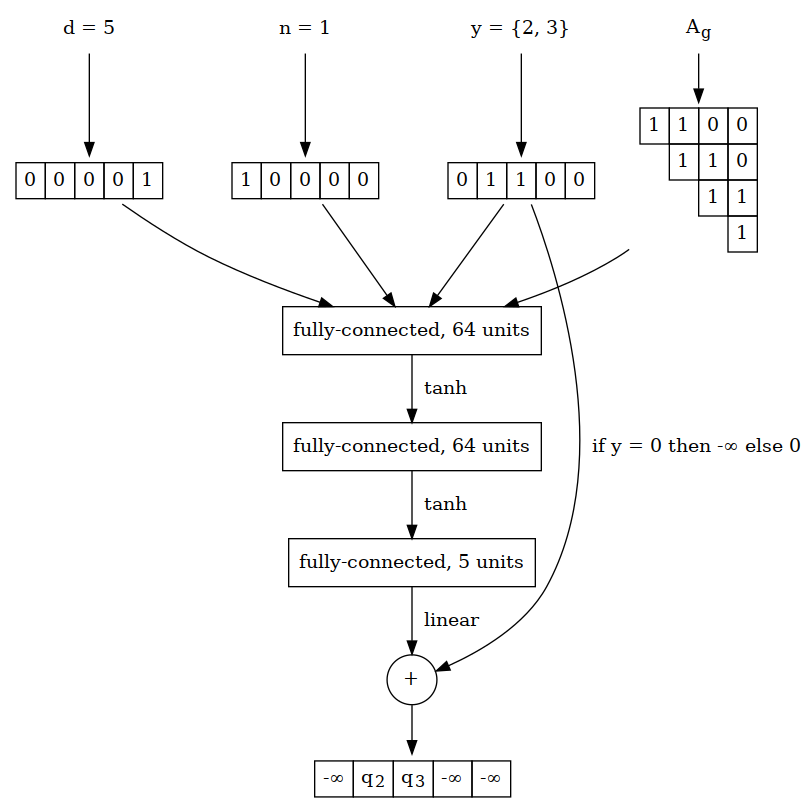
\includegraphics[scale=0.5]{nn-2}
\end{figure}

Базовой частью любого текущего состояния $s$ (или, точнее \textit{наблюдения}
$o \in \Omega$) будем считать кортеж $(n, d, y_1 ... y_m)$, где $n$ --- это
идентификатор (номер) текущего узла, $d$ --- номер узла назначения текущего
пакета, а $y_1 ... y_m$ --- номера соседей текущего узла. Добавление номера
текущего узла позволит одной и той же нейросети работать в качестве роутера в
любом из узлов графа.

Также на вход нейросети подается матрица смежности графа, разложенная в вектор.
Информацию о текущей топологии сети агент получает при помощи алгоритма link-state.

Чтобы избежать взаимозависимости оценок Q-функции для узлов с близкими номерами, будем
использовать \textit{унитарный код}, т. е. для сети с семью узлами номер 3 будет
кодироваться как 0010000, номер 5 --- как 0000100, и т. д. Для кодирования
множества соседей будем использовать тот же принцип, т. е. множество соседей 1,
3, 4 будет закодировано как 1011000. Таким образом, размер базового входного
состояния для нейросети составит $3n$, где $n$ --- количество узлов в сети.

Выходной слой нейронной сети состоит из $n$
нейронов с линейными функциями активации, где $i$-ый нейрон
соответствует $i$-ому узлу в сети. К выходам узлов, не являющихся соседями
текущего, отдельно прибавляется $-\infty$ (на практике --- большое отрицательное
число, например -1000000). Таким образом, на выходе нейросети образуются оценки
функции $Q(s, a)$ для всех действий $a$, где для действий, недоступных в текущем
состоянии (узлов, не являющихся соседями), $Q(s, a) = -\infty$.

\section{DQN-LE-routing}

\begin{figure}[!h]
  \caption{DQN-LE-routing: архитектура сети}\label{nn-1-one-out}
  \centering
  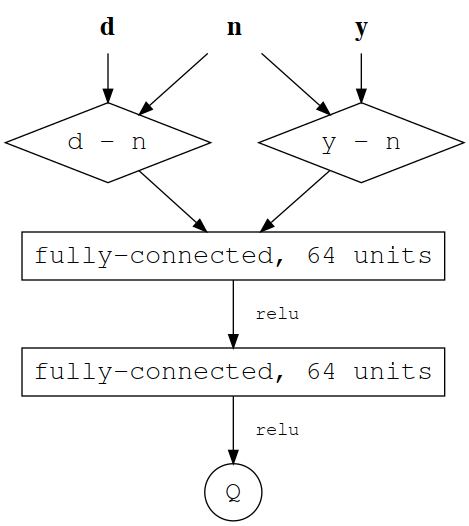
\includegraphics[scale=0.5]{nn-1-one-out}
\end{figure}

TBD

\chapterconclusion

TBD

\chapter{Эксперименты}\label{experiments}

Экспериментальное сравнение разработанных алгоритмов проводилось в двух
имитационных моделях: модели абстрактной компьютерной сети и модели конвейерной
системы. Эксперименты в модели абстрактной компьютерной сети использовались для
того, чтобы проверять работоспособность базовой структуры рассматриваемого
алгоритма в относительно простом сеттинге. Кроме того, симуляция компьютерной
сети является менее вычислительно интенсивной задачей, чем симуляция конвейерной
системы. Также, существуют хорошо изученные способы генерации случайных графов,
обладающих топологическими свойствами, аналогичными таковым у реальных
компьютерных сетей (например, модель Барабаши-Альберт
\cite{albert2002statistical}), в то время как случайная генерация правдоподобных
моделей конвейерной сети является нетривиальной нерешенной задачей. Все это
делает модель компьютерной сети хорошей площадкой для первичного анализа
разработанного алгоритма.

Стоит, однако, подчеркнуть, что рассматривается модель \textit{абстрактной}
компьютерной сети. Отличие рассматриваемой модели от модели реальной
компьютерной сети заключается в том, что служебные сообщения передаются между
узлами мгновенно, в отличие от целевых пакетов, которые испытывают задержку при
проходе по соединениям и в очередях обработки на узлах. Это сделано для того,
чтобы приблизить модель абстрактной компьютерной сети к модели реальной
конвейерной сети.

При проведении экспериментов в обоих моделях разработанные алгоритмы
сравнивались со следующими бейзлайнами:
\begin{itemize}
  \item \textbf{Shortest paths (SP)}: aлгоритм кратчайших путей, использующий протокол link-state; 
  \item \textbf{Q-routing}, описанный в разделе \ref{q-routing-desc} и
    являющийся идейным предком предложенных алгоритмов DQN-routing и DQN-LE-routing.
  \item TBD: добавить бейзлайны
\end{itemize}

Каждый тестовый сценарий для каждого типа алгоритма был запущен трижды с
различными числами инициализации генератора случайных чисел (были использованы
числа 42, 43 и 44). Целевые значения усреднялись на временных отрезках в 500
единиц времени модели. На представленных графиках линиями представлены значения,
усредненные по трем запускам сценария; соответствующими линиям полупрозрачными
полосами изображены разбросы между минимальным и максимальным значениями по трём
запускам.

\section{Эксперименты в модели абстрактной компьютерной сети}\label{experiments:network}

Нейросетевые агенты для алгоритмов DQN-routing и DQN-LE-routing перед работой
проходили предварительное обучение с учителем на эпизодах работы алгоритма
кратчайших путей внутри графа из 10 вершин (Рис.~\ref{fig-simple-network}).
Каждое соединение в графе имеет задержку 10 мс и пропускную способность 1024 байт/мс.
Каждый пакет имеет размер 1024 байт, каждый роутер обрабатывает один пакет за 5
мс. Алгоритм кратчайших путей в качестве веса ребра использует его задержку.

Всего было сгенерировано 230000 эпизодов, включая эпизоды работы на версиях
данного графа с некоторыми отсутствующими ребрами. Для DQN-LE агента
использовались графовые эмбеддинги размерности 8. Оба нейросетевых агента
обучались на данных в течение 10 эпох с помощью алгоритма RMSProp \cite{tieleman2012lecture}.

\begin{figure}[!h]
  \caption{Базовый граф для тестов в модели компьютерной сети}\label{fig-simple-network}
  \centering
  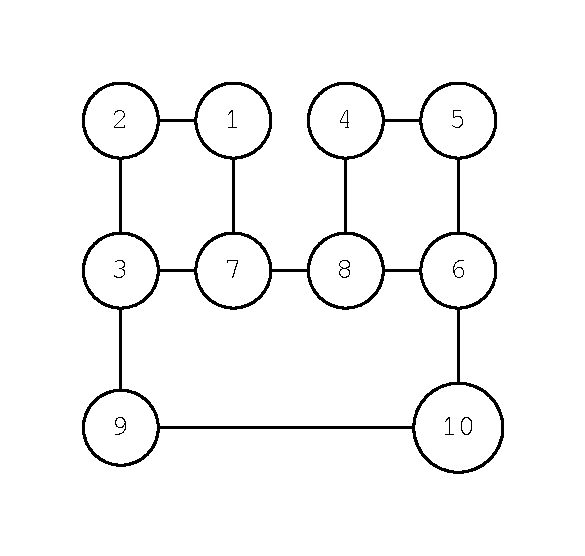
\includegraphics[scale=0.6]{graph-2.pdf}
\end{figure}

\subsection{Адаптация к изменениям интенсивности трафика}

\begin{figure}[!h]
  \caption{Резкое понижение и последующее снижение нагрузки}\label{experiments:network:peak-load-small}
  \centering
  \includegraphics[width=\textwidth]{peak-load-small}
\end{figure}

В этом сценарии пакеты перемещаются между двумя половинами
графа \ref{fig-simple-network} (между множествами вершин $\{1, 2, 3, 7\}$ и
$\{4, 5, 6, 8\}$). Сначала пакеты посылаются раз в 10 мс, затем нагрузка резко
возрастает --- пакеты посылаются с периодом 3.5 мс ---, и в конце падает вновь.

В условиях повышения нагрузки на сеть и перегрузки <<популярных>> роутеров,
через которые проходит большинство кратчайших путей (узлы 7 и 8 в графе
\ref{fig-simple-network}) алгоритм shortest paths не способен работать эффективно,
как видно на графике \ref{experiments:network:peak-load-small} --- очереди этих
роутеров начинают стремительно расти, а с ними и среднее время доставки пакетов.
Все прочие алгоритмы оказываются способны быстро обнаружить затор и повести
трафик обходным путём.

\subsection{Изменение топологии сети}\label{experiments:simple/links}

\begin{figure}[!h]
  \caption{Обрыв и последующее восстановление трех соединений}\label{experiments:network:topology-change-small}
  \centering
  \includegraphics[width=\textwidth]{topology-change-small}
\end{figure}

В этом сценарии при небольшой нагрузке в сети производился последовательный
обрыв соединений $(7, 8)$, $(1, 2)$ и $(5, 6)$ и последующее их восстановление в том
же порядке. Пакеты посылались, как и в предыдущем сценарии, между двумя
половинами графа \ref{fig-simple-network}.

Как видно на графике \ref{experiments:network:topology-change-small}, алгоритмы
DQN- и DQN-LE-routing в этом сценарии работают почти в точности так же, как и
оптимальный в этой ситуации алгоритм кратчайших путей, в то время как Q-routing
не способен вернуться к оптимальному поведению после восстановления всех
соединений.

\subsection{Перенос опыта на новые топологии графов}

Необходимость предобучения для работы в графе заданной топологии является
существенным недостатком алгоритма DQN-routing, сильно ограничивающим его
практическую ценность. Алгоритм DQN-LE-routing тоже требует предобучения, но
благодаря использованию графовых эмбеддингов обобщающая способность единожды
обученной модели гораздо выше.

\begin{figure}[!h]
  \caption{Случайный граф из 10 вершин}\label{fig-random-net-10n}
  \centering
  \includegraphics[scale=0.7]{random-graph-10n}
\end{figure}

Нейросетевые агенты для алгоритмов DQN- и DQN-LE-routing, обученные на данных с
базового графа из 10 вершин (рис. \ref{fig-simple-network}), были использованы
для работы в случайном графе из 10 вершин, сгенерированном по модели
Барабаши-Альберт с параметром $m = 2$ и случайными значениями задержки
соединений от 10 до 20 мс. Прочие параметры сгенерированного графа идентичны
таковым в базовом графе. 

\begin{figure}[!h]
  \caption{Перенос опыта на новую топологию графа}\label{experiments:network:transfer-small}
  \centering
  \includegraphics[width=\textwidth]{learning-transfer-small}
\end{figure}

График \ref{experiments:network:transfer-small} демонстрирует показатели работы
алгоритмов в новом графе при низкой нагрузке. Работа алгоритма кратчайших
путей (оптимального при низкой нагрузке) также приведена для сравнения. Видно,
что DQN-routing ведет себя в новом графе хаотично и даже не способен сойтись к
какой-либо стабильной стратегии. В отличие от него, DQN-LE-routing работает
оптимально (аналогично алгоритму кратчайших путей) с самого начала, что
позволяет сделать вывод, что опыт нейросети, полученый при обучении, очень
хорошо обобщается на графы того же размера.

\begin{figure}[!h]
  \caption{Случайный граф из 40 вершин}\label{fig-random-net-40n}
  \centering
  \includegraphics[scale=0.7]{random-graph-40n}
\end{figure}

\begin{figure*}[!h]
  \centering
  \subfloat[Низкая нагрузка]{
    \includegraphics[width=0.4\textwidth]{learning-transfer-big-low-load}
    \label{experiments:network:transfer-big-low}}
  \hfil
  \subfloat[Высокая нагрузка]{
    \includegraphics[width=0.4\textwidth]{learning-transfer-big-high-load}
    \label{experiments:network:transfer-big-high}}
  \caption{Перенос опыта на новую топологию большего размера}\label{experiments:network:transfer-big}
\end{figure*}

Нейросетевой агент алгоритма DQN-routing, обученный на графе с $N$ вершинами,
принципиально не может работать на графах большего размера, однако
DQN-LE-routing свободен от этого ограничения, так как векторные представления
заданной размерности $d$ можно получить для вершин любого графа. На графиках
\ref{experiments:network:transfer-big-low} и
\ref{experiments:network:transfer-big-high} изображена работа алгоритма
DQN-LE-routing, предобученного на базовом графе из 10 вершин, внутри случайного
графа из 40 вершин (рис. \ref{fig-random-net-40n}), в условиях низкой и высокой
нагрузки. В условиях низкой нагрузки DQN-LE-routing начинает показывать
приемлемое качество работы существенно быстрее, чем Q-routing, хоть и не
сходится к оптимальной стратегии аналогичной алгоритму кратчайших путей --- но к
ней не может сойтись и Q-routing. В условиях высокой нагрузки DQN-LE-routing
ведет себя существенно лучше обоих бейзлайнов --- shortest path переполняет
очереди ключевых узлов и расходится, Q-routing долгое время ведет себя хаотично,
прежде чем сойтись к очень неоптимальной стратегии, в то время как
DQN-LE-routing работает как часы.

Из результатов экспериментов можно сделать вывод, что предобученный DQN-LE-routing обладает
хорошей обобщающей способностью и способен успешно работать на большом множестве
различных графов.

\section{Эксперименты в модели конвейерной системы}\label{experiments:conveyors}

В отличие от модели компьютерной сети, в модели конвейерной системы алгоритм
будет пытаться оптимизировать не только среднее время доставки пакета
(чемодана), но и \textit{энергопотребление} конвейеров. Оптимизация
энергопотребления заключается в том, чтобы использовать для доставки чемоданов
до точек назначения как можно меньше конвейеров.

В алгоритме DQN-routing на вход нейросети будет дополнительно подаваться вектор
$w$ размера $n$ (где $n$ --- количество конвейерных секций в системе), в котором на $i$-ой
позиции стоит 0, если конвейер, на котором находится секция $i$, в данный момент
находится в состоянии ожидания, и 1 --- если он работает.

В алгоритме DQN-LE-routing при расчете Q-функции для соседней секции $x$ на вход
нейросети будет дополнительно подаваться число 1, если конвейер, на котором
находится секция $x$, работает, и 0 --- если не работает.

Эксперименты проводились на модели конвейерной сети из 14 конвейеров с 27
секциями в сумме, двумя входными вершинами и четырьмя выходными вершинами (рис.
\ref{test-conveyors}). Секции с первой по 20 имеют длину 10 метров, с 21 по 27 --- 2
метра. Энергопотребление каждого конвейера равно 1 кВт, максимальная
скорость --- 1 м/c.

\begin{figure}[!h]
  \caption{Модель конвейерной системы для тестов}\label{test-conveyors}
  \centering
  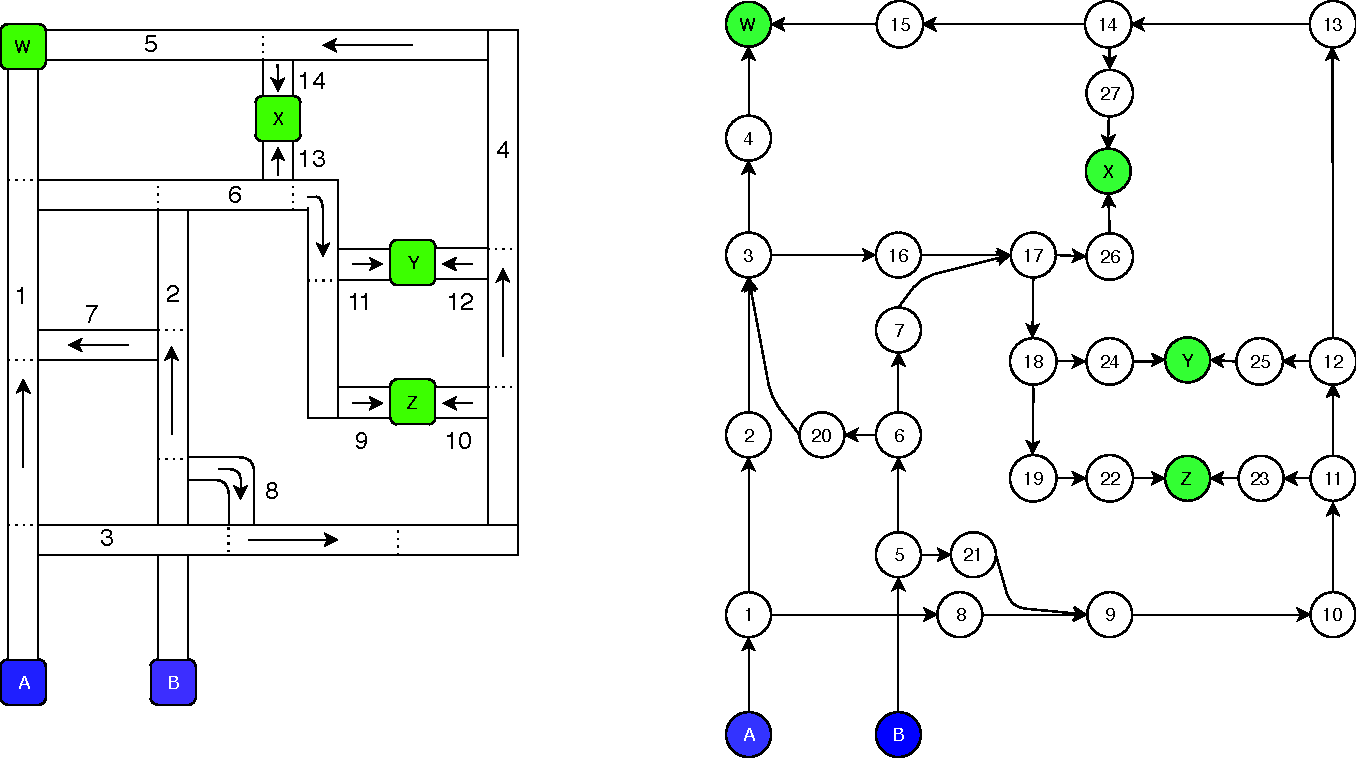
\includegraphics[scale=0.5]{test-conveyors}
\end{figure}

\subsection{Неравномерный поток до выходных вершин}

Как можно видеть на иллюстрации \ref{test-conveyors}, кратчайший путь от входов
до выходов W и X пролегает через конвейеры 1, 2, 7 и 6, а до выходов Y и Z --
через конвейеры 1, 2, 3 и 4. Однако до выходов Y и Z также можно попасть через
конвейер 6, не задействуя конвейеры 3 и 4. Если для нас важно оптимизировать
энергозатраты, то в условиях небольшого входящего потока чемоданов такая
стратегия является более предпочтительной.

\begin{figure*}[!h]
  \centering
  \subfloat[Время сумок в пути]{
    \includegraphics[width=0.4\textwidth]{conveyors1-time}
    \label{experiments:conveyors:1-time}}
  \hfil
  \subfloat[Энергопотребление системы]{
    \includegraphics[width=0.4\textwidth]{conveyors1-energy}
    \label{experiments:conveyors:1-energy}}
  \caption{Неравномерный поток до выходных вершин}\label{experiments:conveyors:1}
\end{figure*}

В данном сценарии поток чемоданов попеременно идет либо только в выходы W и X,
либо во все четыре выхода сразу. Параметр важности экономии энергопотребления
$\alpha$ равен 1.

На иллюстрации \ref{experiments:conveyors:1} видно, что алгоритмы DQN- и
DQN-LE-routing после непродолжительного периода адаптации начинает работать
заметно лучше алгоритмов shortest paths и Q-routing с точки зрения экономии энергии,
жертвуя средним временем доставки чемодана. 

\subsection{Плавное повышение нагрузки}

\begin{figure*}[!h]
  \centering
  \subfloat[Время сумок в пути]{
    \includegraphics[width=0.4\textwidth]{conveyors2-late-time}
    \label{experiments:conveyors:2-late-time}}
  \hfil
  \subfloat[Энергопотребление системы]{
    \includegraphics[width=0.4\textwidth]{conveyors2-late-energy}
    \label{experiments:conveyors:2-late-energy}}
  \caption{Плавное повышение нагрузки: $\alpha = 1$, $\alpha_{LE} = 0.4$}\label{experiments:conveyors:2-late}
\end{figure*}

Первая половина этого сценария повторяет предыдущий --- поток попеременно идет то
во все выходы, то только в выходы W и X. Во второй половине сценария частота
появления чемоданов на входах возрастает в два раза и продолжает плавно расти.

В этом сценарии алгоритмы DQN- и DQN-LE-routing используют разные параметры
важности экономии энергопотребления, обоначенные соотв. $\alpha$ и
$\alpha_{LE}$, так как на практике алгоритм DQN-LE-routing оказался более
чувствительным к величине этого параметра.

\begin{figure*}[!h]
  \centering
  \subfloat[Время сумок в пути]{
    \includegraphics[width=0.4\textwidth]{conveyors2-early-time}
    \label{experiments:conveyors:2-early-time}}
  \hfil
  \subfloat[Энергопотребление системы]{
    \includegraphics[width=0.4\textwidth]{conveyors2-early-energy}
    \label{experiments:conveyors:2-early-energy}}
  \caption{Плавное повышение нагрузки: $\alpha = 0.8$, $\alpha_{LE} = 0.2$}\label{experiments:conveyors:2-early}
\end{figure*}

Графики \label{experiments:conveyors:2-late}
и \label{experiments:conveyors:2-early} показывают, что при постепенном
увеличении интенсивности трафика (и, как следствие, загруженности конвейеров)
алгоритмы DQN- и DQN-routing в какой-то момент начинают использовать конвейеры 3
и 4, чтобы снизить среднюю скорость доставки чемоданов, причем это происходит
тем раньше, чем ниже параметр $\alpha$ ($\alpha_{LE}$).

\chapterconclusion

TBD

%% Макрос для заключения. Совместим со старым стилевиком.
\startconclusionpage

TBD

%% Обратите внимание на heading. Без него тоже работает, но название будет другим.
\printmainbibliography

%% После этой команды chapter будет генерировать приложения, нумерованные русскими буквами.
%% \startappendices из старого стилевика будет делать то же самое
\appendix

\chapter{Промежуточные результаты исследования}\label{apx:bad-results}

TBD

\chapter{Описание разработанных имитационных моделей}\label{apx:simulators}

TBD                

\end{document}
